
\newcommand{\etas}{\ensuremath{\eta_{\mathrm{s}}}}


\chapter{Introduction}

The rise of cryptocurrencies have openend up unending possibilities of how minimal or no trust based systems could be established owing to decentralization.
The concept of blockchain was introduced with the founding of Bitcoin by Satoshi Nakamoto \cite{Nakamoto2009}.
Satoshi Nakamoto proposed and implemented idea of a consensus based, trustless, truly peer-to-peer system for financial transactions.  
Notwithstanding an intrumental step towards establishing a decentralized and a trustless system, Bitcoin has several practical limitations with regards to privacy, security and scalability \cite{Conti2018}.   
This led to the development of more privacy and anonymity focussed cryptocurrencies like Monero \cite{Saberhagen2013} and Zcash \cite{Sasson2014}.
Grin \cite{GrinWebsite} and Beam \cite{BeamWebsite} are two relatively new projects which are backed by the MimbleWimble protocol \cite{Poelstra2016} and claim to promise scalability, anonymity and fungibility all at once.
The rise in privacy-centric cryptocurrencies further led to growth in popularity of cryptocurrencies not only among investors but also common people.


\section{What is a Blockchain?}
\label{scn:blockchain}

The concept of a Blockchain originates from the idea of having a decentralized, publicly visible and trust-free ledger.
The term \textit{blockchain} was first coined by Satoshi Nakamoto, the creator of Bitcoin \cite{Nakamoto2009}.
In literal terms, a blockchain implies that blocks containing financial transactions would be added to a publicly verifiable ledger in a timely manner, forming a \textit{chain} of \textit{blocks}.
We expand on the need and the basic idea of a decentralized ledger in the following subsection.

\subsection{Decentralized Ledger}

A ledger is a principal book of records which keeps a track of all transactions measured in terms of a monetary unit. Bitcoin is a decentralized, public ledger, decentralized because there is no trusted third party controlling the ledger and public because anyone with bitcoin can participate in the network, receive and send bitcoins, and even hold a copy of this ledger (essentially, the history of all transactions) if they want to. In that sense, the ledger is "non-trusted" and transparent to public. As opposed to such a decentralized ledger setup, traditional banks use centralized ledger system where each bank has it's own ledger visible only to the concerned user.\\ 

\begin{figure}[h!]
    \centering
    \begin{subfigure}[b]{0.5\textwidth}
        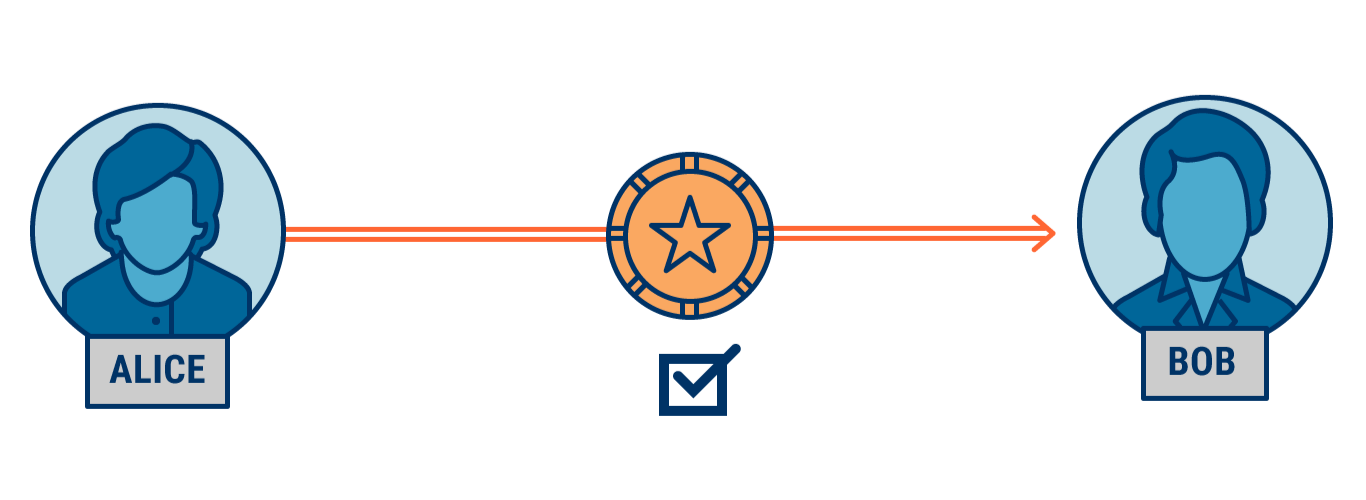
\includegraphics[width=\textwidth]{Figures/blockchain1.png}
        \caption{A physical transaction}
        \label{fig:bc1}
    \end{subfigure}
    ~
    \begin{subfigure}[b]{0.5\textwidth}
        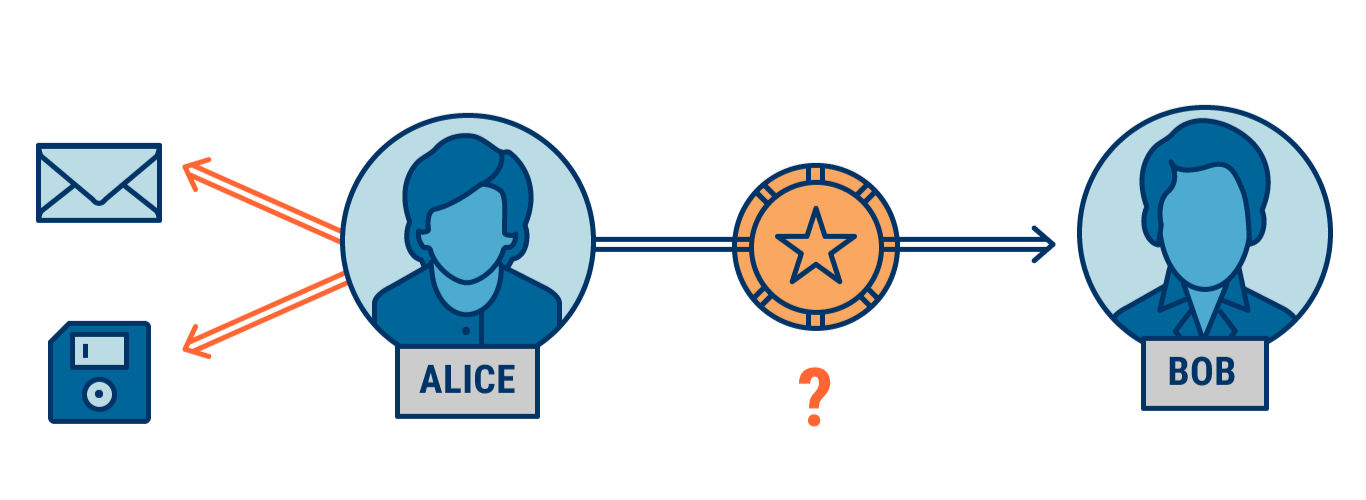
\includegraphics[width=\textwidth]{Figures/blockchain2.png}
        \caption{A digital transaction}
        \label{fig:bc2}
    \end{subfigure}
    ~
    \begin{subfigure}[b]{0.5\textwidth}
        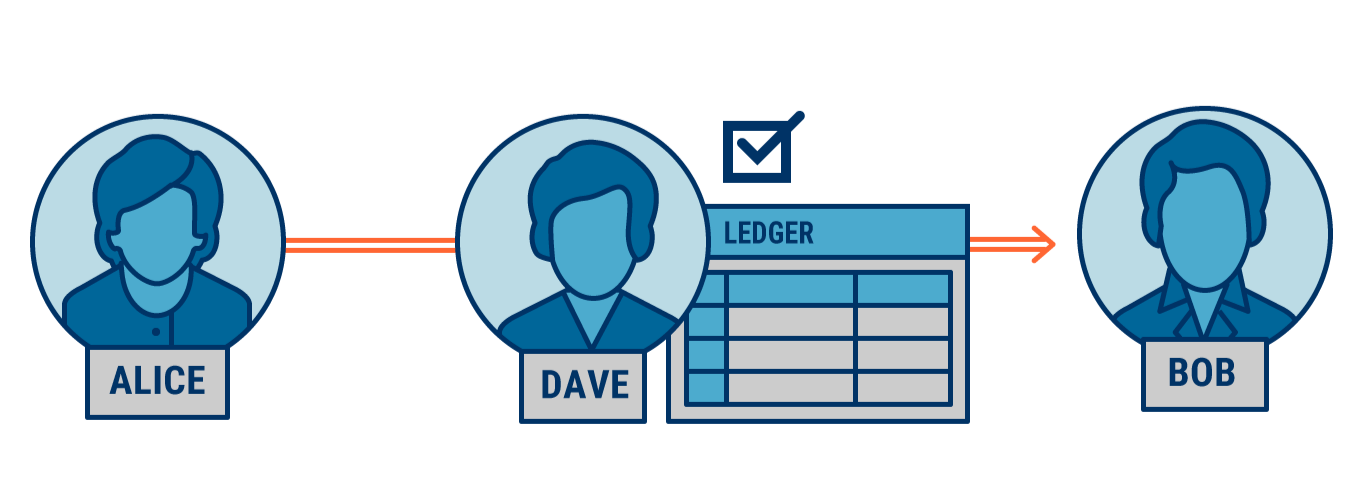
\includegraphics[width=\textwidth]{Figures/blockchain3.png}
        \caption{A digital transaction with ledger}
        \label{fig:bc3}
    \end{subfigure}
    ~
    \begin{subfigure}[b]{0.7\textwidth}
        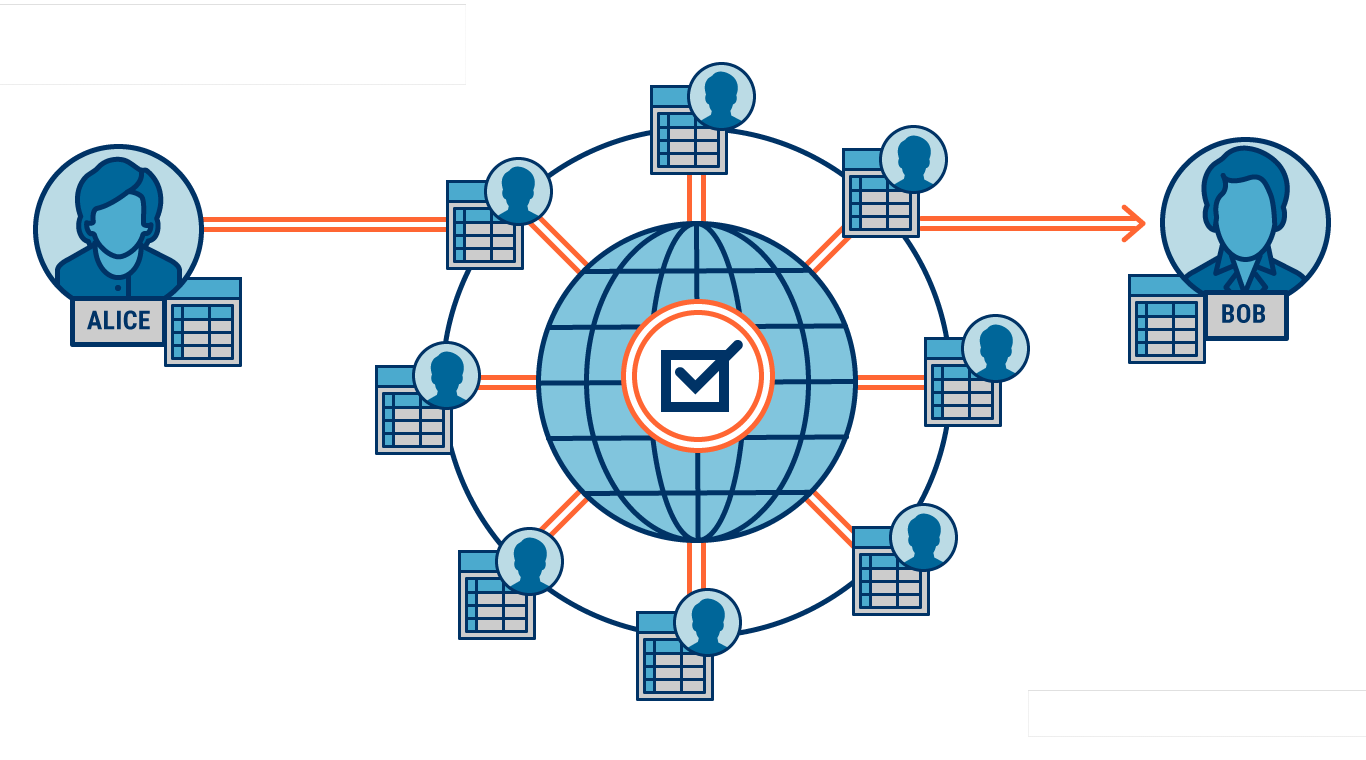
\includegraphics[width=\textwidth]{Figures/blockchain4.png}
        \caption{A decentralized ledger}
        \label{fig:bc4}
    \end{subfigure}
    \caption{Understanding decentralized ledger}
    \label{fig:bc}
\end{figure}

In reference to Figure\footnote{Credits: \url{https://www.cbinsights.com/research/what-is-blockchain-technology/}}
\ref{fig:bc1}, in a physical transaction, the Alice hands Bob a physical arcade coin. Bob now has one coin, and Alice has zero. The transaction is complete. 
If the same transaction is to be performed digitally (Figure \ref{fig:bc2}), Alice would send a string of some bits (corresponding to the desired amount) to Bob. 
Now, since it is just a string of bits, what is the guarantee that Alice would not reproduce that same string of bits in her mail or hard-disk?
If this happens, it would mean that although Alice sent Bob the amount, Alice still possesses the same amount. 
This clearly is a violation.
To tackle this, we must have a ledger or a record of all transactions between Alice and Bob. 
When Alice gives Bob the digital token, the ledger records the transaction (Figure \ref{fig:bc3}). 
Bob has the token, and Alice does not. Let us call the one who maintains this ledger as Dave.
This setup assumes that Dave is a trusted middleman for maintaining ledger. 
Now, what if Alice bribes Dave to erase her transaction? What if Dave decides to charge a fee that neither Alice or Bob want to pay? 
What happens when Alice and Bob cannot trust the third party? This results in a decentralized and public ledger system (Figure \ref{fig:bc4}). 
When a lot of people have a copy of the same ledger, it becomes very difficult to tamper the system and cheat. 
This works because everyone is holding a copy of the same digital ledger and more the number of trusted people holding this ledger, the stronger it becomes.


Blockchain technology offers a way for untrusted parties to reach a consensus on a common digital history. The World Bank defines Blockchain as follows \cite{natar17}:

\begin{defn}[Blockchain]
    A 'blockchain' is a particular type of data structure used in some distributed ledgers
    which stores and transmits data in packages called "blocks" that are connected to each
    other in a digital 'chain'. 
\end{defn}

Blockchains employ cryptographic algorithms to record and synchronize data across a network in an unchangeable manner. The \textit{state} of the Blockchain is the current status of the ledger visible to public. 
In case of Bitcoin, any independent observer can verify the state of the blockchain as well as the validity of all the transactions on the ledger.
This is a \textit{serious} limitation for Bitcoin and could possibly prohibit many use cases.
As an example, if employees of a company were to receive their salaries in bitcoin, would they agree if their salaries were published on the public blockchain? 
This naturally demands for a transaction system which preserves \textit{anonymity} and \textit{confidentiality}.


\section{Notion of Privacy on a Blockchain}

The very concept of having all the information about transactions (predominantly financial) public via a distributed ledger or a blockchain demands for privacy and anonymity of the users.
Before we talk about privacy on the blockchain, it is necessary to understand what we do mean by terms like \textit{privacy} and \textit{anonymity}.
Modern day cryptography is based on the following primary functions \cite{kesler98}:
\begin{enumerate}
    \item[(i)] \textit{Privacy/confidentiality}: To ensure that no one can read or access the message except the intended receiver
    \item[(ii)] \textit{Authentication}: Proving one's identity
    \item[(iii)] \textit{Integrity}: Ensuring that the message intended to be received by the receiver is not altered in the path
    \item[(iv)] \textit{Non-repudiation}: A protocol for checking if a message was actually generated by the sender
    \item[(v)] \textit{Key exchange}: The protocol which determines how key(s) are shared between the sender and the receiver
\end{enumerate}

All of the above functions form an necessary part of a cryptographic system. A well-designed system ensures all of the above functions are taken care of considering the computational bounds for carrying out any protocol.
In a confidential transaction, it is desirable to have \textit{confidentiality} and \textit{anonymity}. 
This means that in a valid confidential transaction, the identity of the sender and receiver must be confidential and the amounts transferred must also be hidden. 
The idea of having such private transactions in digital currencies could be traced back to David Chaum's work on blind signatures \cite{chaum82}.
A similar concept of privacy is required in the blockchain framework. 
The digital assets owned by users must not be publicly visible.
There should be a mechanism to unlink the identity of a user with his or her digital identity, i.e. public key address. 
The interaction between the sender and the receiver in a transaction must not reveal anything to them other than the amounts being transferred.
A user must not be able to reuse his or her digital assets. 
Making the transactions digital and public at the same time brings about several challenges in ensuring that the above requirements are being satisfied.
Active research is still being pursued in the direction of not only solving such practical problems but to do them efficiently and in a scalable manner.

\section{Cryptocurrency Exchanges \& Security}



\section{Proof of Solvency}

\subsection{Proof of Reserves}
\subsection{Proof of Liabilities}



%%


%%% Local Variables: 
%%% mode: latex
%%% TeX-master: "../mainrep"
%%% End: 
